\documentclass[letterpaper,9pt,twocolumn,twoside,]{pinp}

%% Some pieces required from the pandoc template
\providecommand{\tightlist}{%
  \setlength{\itemsep}{0pt}\setlength{\parskip}{0pt}}

% Use the lineno option to display guide line numbers if required.
% Note that the use of elements such as single-column equations
% may affect the guide line number alignment.

\usepackage[T1]{fontenc}
\usepackage[utf8]{inputenc}

% pinp change: the geometry package layout settings need to be set here, not in pinp.cls
\geometry{layoutsize={0.95588\paperwidth,0.98864\paperheight},%
  layouthoffset=0.02206\paperwidth, layoutvoffset=0.00568\paperheight}

\definecolor{pinpblue}{HTML}{185FAF}  % imagecolorpicker on blue for new R logo
\definecolor{pnasbluetext}{RGB}{101,0,0} %


\usepackage{booktabs}
\usepackage{longtable}
\usepackage{array}
\usepackage{multirow}
\usepackage{wrapfig}
\usepackage{float}
\usepackage{colortbl}
\usepackage{pdflscape}
\usepackage{tabu}
\usepackage{threeparttable}
\usepackage{threeparttablex}
\usepackage[normalem]{ulem}
\usepackage{makecell}

\title{Persistence and Change in Attitudes Toward Unification with North
Korea}

\author[a]{Sanghoon Park}
\author[b]{Jaeyoung Hur}

  \affil[a]{Department of Political Science, University of South
Carolina, SC, USA}
  \affil[b]{Global leaders College, Yonsei University, Seoul, ROK}

\setcounter{secnumdepth}{0}

% Please give the surname of the lead author for the running footer
\leadauthor{Park and Hur}

% Keywords are not mandatory, but authors are strongly encouraged to provide them. If provided, please include two to five keywords, separated by the pipe symbol, e.g:
 \keywords{  The Panmunjom Declaration |  Attitudes on Korean
Unification |  Attitudes toward North Korea |  Generations |  Prospects
of unification  }  

\begin{abstract}
This article examines whether existing explanations of South Korean
attitudes regarding North Korea and Korean unification adequately
explain changes after the declaration at Panmunjom on April 27, 2018.
This study uses the National Consciousness Survey Data to estimate these
shifts in attitude. Our results show that South Korean attitudes shifted
following the Panmunjom Declaration for Peace, Prosperity, and
Unification of the Korean Peninsula. We show that existing explanations
for generational effects do not explain the national attitude shifts on
unification; our study demonstrates that a wide divergence exists
between younger and the older generations, and younger generations are
more likely to display a negative attitude toward North Korea and
unification even after the Declaration. We also show that the prospects
of unification evoke different attitudes across generations. Our results
imply that the Panmunjom Declaration is a prominent political event, but
it is necessary to analyze it without overestimating it.
\end{abstract}

\dates{This version was compiled on \today} 


% initially we use doi so keep for backwards compatibility
% new name is doi_footer

\pinpfootercontents{Manuscripts}

\begin{document}

% Optional adjustment to line up main text (after abstract) of first page with line numbers, when using both lineno and twocolumn options.
% You should only change this length when you've finalised the article contents.
\verticaladjustment{-2pt}

\maketitle
\thispagestyle{firststyle}
\ifthenelse{\boolean{shortarticle}}{\ifthenelse{\boolean{singlecolumn}}{\abscontentformatted}{\abscontent}}{}

% If your first paragraph (i.e. with the \dropcap) contains a list environment (quote, quotation, theorem, definition, enumerate, itemize...), the line after the list may have some extra indentation. If this is the case, add \parshape=0 to the end of the list environment.


\hypertarget{introduction}{%
\subsection{Introduction}\label{introduction}}

The unification policy in South Korea has been up and down with various
handovers of administration. Conservative administrations tended to take
a strong stance against North Korea, while liberal administrations led
the engagement policy as a basis for reconciliation and cooperation.
President Jae-In Moon, elected in a shift of power from the conservative
administration over the past decade, is leading the inter-Korean
relationship to a new phase. The new administration is pushing for
policies that require inter-Korean cooperation, which was not the case
under the conservative administration. For instance, the inter-Korean
relationship is rapidly changing in political, cultural, and military
policies, such as the joint inter-Korean rail investigation, the
withdrawal of the demilitarized zone guard post (DMZ GP), the linkage of
the arrowhead roads in DMZ for the KIA (Killed in Action) Recovery and
Identification project, and the promotion of forest cooperation.

Indeed, the inter-Korean relationship faced several historical events in
2018. North Korea sent athletes, cheering squads, and art troupes to the
Pyeongchang Winter Olympics. After alleviating these tensions and
creating an atmosphere of cooperation, South Korea and North Korea held
three summit meetings together. The series of meetings led to the
Panmunjom Declaration on April 27, and the Pyongyang Joint Declaration
on September 19. Similarly, incumbent leaders of the United States and
North Korea held their first summit in history. At the first meeting,
between the US and North Korea, the leaders adopted the Singapore Joint
Statement, promising a joint effort to build a lasting and substantial
peace regime on the Korean peninsula. US--North Korea relations, as well
as inter-Korean relations, are on a new path, and we are in a unique
international situation concerning the Korean Peninsula.

Do the recent changes fundamentally address North Korea's ongoing threat
to the security of South Korea and inter-Korean relations? In other
words, the question is whether the Panmunjom Declaration is meaningful
enough to change the inter-Korean relationships fundamentally like the
previous declarations, such as the South-North Joint Declaration in June
2000, and the North--South Summit Declaration in October 2007. Existing
studies have explained the differences of opinions of Korean people
toward the unification issues in terms of political ideology and
generation. However, members of Korean society have experienced various
policy changes and the development of national guidance from North
Korea. One can question whether the changes caused by the Panmunjom
Declaration will lead to the same results as previous declarations.

For the Pyeongchang Winter Olympics of 2018, 80\% of Koreans in their
20s and 30s opposed the formation of the joint South Korean and North
Korean women's ice hockey team \citep{SeongHong2018}. The ``National
Consciousness Survey on Inter-Korean Integration 2017,'' published by
the Korea Institute for National Unification, found that negative
attitudes toward the need for unification, unification tax, and expected
benefits for unification were significantly higher for Koreans in their
20s and 30s than for other age groups. Besides this, respondents were
divided as to whether they regarded the two Koreas as a single nation.
This change paradoxically shows that we need to consider unification
issues from different perspectives for a changing future, and suggests
that existing theoretical analysis needs to reconsider whether they are
producing meaningful results under such changing contexts.

This study examines whether the political event of the Panmunjom
Declaration has changed the attitudes and perceptions of Korean people
toward unification. If the Panmunjom Declaration is indeed a significant
event, we can observe rapid changes in attitudes and perceptions toward
inter-Korean relationships, which might affect the success or failure of
future policies. As a result, it is difficult to say that the event has
changed the attitudes toward North Korea and unification after the
Panmunjom Declaration. It means that the Panmunjom Declaration might not
fundamentally change the long-term view of respondents on inter-Korean
relations.

This paper is organized as follows. In the next two sections, we review
the theoretical and empirical studies on the issues of unification and
North Korea relations. In Section 4, we develop the conceptual framework
of our analysis. Following this, Section 5 describes the dataset and
empirical models we have constructed to test our hypotheses about
changes after the Panmunjom Declaration. Section 6 presents and
discusses our empirical results, and we conclude by addressing issues
for further inquiry.

\hypertarget{the-effect-of-political-events-on-attitudes-toward-north-korea-and-unification-in-south-korea}{%
\subsection{The Effect of Political Events on Attitudes toward North
Korea and Unification in South
Korea}\label{the-effect-of-political-events-on-attitudes-toward-north-korea-and-unification-in-south-korea}}

\hypertarget{attitudes-toward-north-korea-and-unification-in-south-korea}{%
\subsubsection{Attitudes toward North Korea and Unification in South
Korea}\label{attitudes-toward-north-korea-and-unification-in-south-korea}}

Since the end of 1998, when the Dae-Jung Kim administration was
attempting to improve inter-Korean relations, scholars have been
actively producing research related to inter-Korean relationships. The
research on inter-Korean relationships is diverse. Some studies discuss
the government's countermeasures related to military provocations.
Others diagnose the nature of a particular administrations' policy
toward North Korea, while still others examine the people's attitudes
toward unification and North Korea policy.

Studies that derive implications through empirical research using
surveys can provide leverage for policymakers. Since these studies
contribute to looking at public attitudes on the issues of unification
and North Korea issues, it helps policymakers establish policy that
corresponds with the demand of the public. For sustainable unification
and North Korea policies, it is necessary to understand the attitudes
toward unification and North Korea of the people at the micro-level.

Many scholars have investigated the changes and trends of South Koreans
using surveys. Some find that respondents' attitudes toward unification
and North Korea differ depending on their political ideologies,
political sophistication, and the level of partisanship. For example,
the more someone has a liberal ideology, the more likely one is to
support the Moo-hyun Rho administration's moderate policy toward North
Korea. At the same time, the more conservative one is, the more likely
one is to advocate the Myung-bak Lee administration's firm policy toward
North Korea \citep{SongKwon2013}.

However, it is an unrealistic assumption that every voter correctly
understands his political ideology. Sophisticated voters will choose to
vote based on their political ideology or policy evaluation, but if
voters are not sophisticated, they are less likely to vote based on
political motivation \citep{Campbell1960, Luskin1984}. In Korean
politics, political sophistication plays a role as a variable that
mediates the political ideology of voters. Only those groups with a high
degree of sophistication show the empirical results of discriminatory
policy preferences in the attitude toward the US-ROK relationship, the
North Korean policy direction, and the North Korean nuclear issues
\citep{Ryu2012}.

Partisanships can be shortcuts for political information or cues, which
can have significant impacts on individual voters' policy preferences.
It is costly for voters to gain proper and precise political
information. When voters obtain specific information to understand any
policy, even a slight increase in costs can be felt. On the other hand,
partisan cues, represented by political parties, help voters to predict
and understand the position of candidates or specific policies, albeit
at a high cost \citep{Rahn1993, Bartels2000, Klar2014}. An empirical
analysis of voters' attitudes toward North Korea policy after the 20th
general election in 2016 shows that supporters of the Democratic Party
felt more efficacy in social and cultural exchange, inter-Korean
economic cooperation, and regular talks than those of the Saenuri Party
\citep{Jung2016}.

There are many studies on the effects of individual tendencies such as
political ideology, political sophistication, and partisanship on an
individual's behavior or personal attitude. However, it is not possible
to clearly explain where these political tendencies come from or what
changes them. In terms of partisanship, \citet{Campbell1960} propose the
concept of party identification, defined as affective orientation.
According to their study, party identification is a psychological
attachment to preferred partisan groups. It is assumed to have an
ongoing tendency, as it is a sort of emotional bond. Thus,
\citet[146--147]{Campbell1960} argue that party identification is formed
in the individual's early socialization process. It implies that
individuals have specific party identification before they reach voting
age. Also, the individuals' nearest social environment, especially the
family, has the most significant influence on forming a party.
\citet[161--165]{Campbell1960} show that the longer the party
identification has been formed, the more the intensity of party
identification increases. In other words, they argue that older
individuals are more likely to enhance their party identifications.
\citet{Bartels2000} also shows that a more substantial influence of
party identification on voting behavior was attributed to the fact that
party identification preceded other political attitudes.

However, while partisanship matters, its influence can vary depending on
its social setting. Here, the social context implies the social
circumstances to which individuals belong. \citet{Klar2014}
disaggregates the partisan differences within groups, because groups are
homogeneous and heterogeneous and between-group variations are
distinctive. \citet{Klar2014} found that within each group, the partisan
gap still holds. In the context of American politics, we can understand
that homogeneous partisan groups which have only Democrats or only
Republicans, have very different partisan effects than heterogeneous
groups, which have a mix of individuals from both parties.

Also, it is possible to consider the possibility that individual voters'
economic considerations will affect unification and North Korea issues.
A simple proposition that voters judge ruling parties when the economy
goes down (or up) theorizes economic voting
\citep{Fiorina1981, Abramowitz2008}. In South Korea, several studies
have revealed that economic voting usually works in presidential
elections \citep{Lee2008, Jang2013, Moon2018}. Reward--punishment
voting, which allows governments and ruling parties to have democratic
accountability to voters, explains how voters' evaluations lead to
voting choice. It suggests that not only can direct economic and
economic downturns at the national and household levels affect how the
people perceive the issues in the future, but they can also affect the
success or failure of specific policies beforehand. For example, the
effects of political events, such as the North--South Summit talks, are
characterized by position issues that are influenced by ideology and
partisanship. In addition, it is closely related to the voter's
retrospective or prospective evaluation \citep{Kim2007}. In the past,
nationalism-based legitimacy mainly explained the issue of unification.

Still, over time, the consideration of the real benefits that can be
achieved by nations and individuals through unification began to emerge
\citep{Choi2016}. The issues related to unification and North Korea are
shifting from a past-oriented approach to a pragmatic approach
\citep{ChoHan2014}. As the division of the two Koreas is prolonged, the
homogeneous national identity is weakened. Therefore, the attitudes
toward unification and North Korea vary, depending on people's
assessment of the realistic political turmoil and economic burden that
unification will bring.

Changes in social composition in the context of the generation--age
cohort may have changed attitudes toward unification and North Korea.
For example, Koreans who were in their 20s during the administrations of
Presidents Dae-Jung Kim and Moo-hyun Roh had a strong tendency to
approve aid to North Korea and oppose preemptive strikes on North Korea.
Other generations that share different social experiences, such as
post-war industrialization or the Korean War, show a distinct tendency
to disagree with aid to North Korea \citep{Chang2018}. Also, the younger
generation in South Korea considers national identity and material
interests at the same time in terms of unification, and they find the
latter more important. It means that attitudes toward inter-Korean
relationship may be affected by a costs-and-benefits consideration. The
negative attitude toward North Korea may be due to the long-term
infarction of inter-Korean relations \citep{ChoHan2014}. Conversely, if
there is a prospect that the benefits of a relationship between the two
Koreas will outweigh the costs, people will likely show a positive
attitude change toward North Korea and unification.

\hypertarget{the-influences-of-political-events}{%
\subsubsection{The Influences of Political
Events}\label{the-influences-of-political-events}}

Political events may occur under highly controlled conditions and can
become predictable. At the same time, political events may occur under
uncontrolled and unpredictable conditions. For example, we can predict
the outcome of a political event such as an election that develops under
a given system and rules. On the other hand, events that occur outside
of the political actors can have unexpected results. Therefore,
political events vary, and the effects of such events also vary
\citep{Smith2005}.

Existing studies have explored what the effects of a political event are
and how it affects different outcomes in various ways. A line of inquiry
examines the direct influence of political events. For instance,
\citet{Smith2005} argues that a politically significant event may
influence the image of political parties. A political event has internal
and external factors. Internal factors make the consumers learn from
events and change the motivations of individual consumers. External
factors are about image power, which is the perception of how
influential the events are.

\citet{Healy2010} attempt to figure out the relationship between
political events and voters' evaluation of the government's performance.
They suggest that political events that people may think are irrelevant
can actually affect the decisions people make on Election Day.
\citet{Healy2010} draw their hypotheses from the psychological
literature that makes an association between voter well-being and
decision-making. They find that a voter with negative information from a
political event may perceive a separate news story about the government
policy in a less positive light \citep[12807]{Healy2010}. These studies
show that political events can be essential information that changes the
motivation of actors and directly affects their political behavior.

Another line of studies focuses on frame building and frame effects.
\citet{Lim2009} present how the US government and the US news media
framed the speech of President George W. Bush in 2002 and how it
affected the public perception of US citizens toward North Korea. The
results show how the frame built by the two counterparts, the government
and the news media, can affect the public's attitudes toward the country
in question. In sum, a political event can affect the motivation of
engaged actors, or a political event is mounted in the hope that it will
be influential. In terms of the latter case, a political event may not
bring fundamental changes.

Theorizing about factors affecting inter-Korean relations is inevitably
influenced by major real-world events surrounding inter-Korean
relationships. In other words, events occurring in North Korea or events
such as a consensus between the two Koreas can drive actual and
theoretical changes by affecting attitudes toward (and images of) North
Korea and unification in South Korean society rather than any other
internal or external changes
\citetext{\citealp[158]{Kim2017}; \citealp{Kim2008}; \citealp{Kim2003}}.

Besides the discussions of existing studies on the attitudes toward
North Korea and unification, we focus on the effect of the Panmunjom
Declaration as a politically critical event. The Panmunjom Declaration
can be understood as a kind of turning point that hints at the
transition in hard policy positions toward unification and North Korea.
Considering the results and outcomes of several official talks with
North Korea in the past, the Panmunjom Declaration may also have
affected people's perception toward North Korea. Before and after the
Panmunjom Declaration, various media suggested the prospect that the
Korean Peninsula issue would develop favorably in the future
\citep{Kim2018b, Smith2018}. After the declaration, President Jae-In
Moon's first year of approval exceeded 80\% \citep{Oh2018, Cho2018}.

When we classify the main events of the inter-Korean relationship into
``conflictive'' versus ``cooperative,'' different types of events would
have differing results in Koreans' attitude toward North Korea and
unification. Conflictive events that cause tensions between the two
Koreas, such as the North Korean nuclear test, may increase the
likelihood that people will show a negative attitude toward North Korea
and unification. On the contrary, events that ease tensions, such as
summit talks, are more likely to reduce the perception of the possible
threat posed by North Korea and to encourage positive attitudes toward
unification. In other words, the main event of the inter-Korean
relationship can influence the attitudes of South Korean society members
\citep[160-161, 171]{Kim2017}. If so, the Panmunjom Declaration can be
an event with the effect of alleviating hostile perceptions of North
Korea, as the summit between South and North Korea, which took place
over ten years after President Myung-Bak Lee's administration imposed
full sanctions against North Korea on May 24, 2010. It implies that we
need to consider whether there has been any significant change in
people's perception of North Korea. In other words, when an incident
creates an atmosphere of reconciliation between the two Koreas, it is
necessary to analyze whether the event fundamentally changed the
understanding of the people who experienced the event.

Members of South Korean society are involved in conflictive or
cooperative events with North Korea. They have experienced policy cycles
in the past two decades in which North and South Korea repeat both
cooperation and conflict. How to judge the success or failure of
policies for managing North Korea can affect South Korean attitudes
toward North Korea and unification. For example, those who believe that
the appeasement policies of previous South Korean administrations toward
North Korea have failed may not expect North Korea to change
substantially despite the Panmunjom Declaration.

The recent tendency that the younger generation in South Korea shows
more conservative attitudes suggests that the same type of events may
have various influences. The characteristics of the young generation,
which have been seen in previous studies such as ``Cooperation with
North Korea, Pro-unification, and Self-Defense,'' have been affected by
conservative characteristics as shown in studies such as ``Strong
against North Korea, Passive or Anti-unification, and Korea-US
Alliance'' \citep{Bae2018}. Since the early 2000s, younger generations
who have experienced tensions between the two Koreas are likely to have
formed a negative perception of and attitudes toward North Korea and
unification \citep{Hur2014}.

\hypertarget{research-design}{%
\subsection{Research Design}\label{research-design}}

\hypertarget{research-hypotheses}{%
\subsubsection{Research Hypotheses}\label{research-hypotheses}}

This study seeks to investigate whether the Panmunjom Declaration
changed the attitude toward North Korea and unification. First, we
explore the determinants of the attitude toward the North Korean
leadership and the attitude toward North Korea in general. On the one
hand, the ministry of defense of South Korea primarily designated as
``enemies'' those which support the hereditary regimes of Il-Sung Kim,
Jong-Il Kim, and Jong-Un Kim of North Korea such as the Communist regime
of the Democratic People's Republic of Korea, paramilitary
organizations, and domestic support in South Korea until 2018. On the
other hand, the Ministry of Unification defines North Korea as a dual
entity. North Korea is not only a political and military confrontation,
but also a partner to cooperate with to build a national community. In
this reality, the two Koreas have maintained hostile relations since the
Cold War yet have sought cooperation to achieve peaceful unification.
\citet{Kim2003} describe the paradoxical attitudes of South Koreans
toward North Korea as ambivalent.

One of the studies on attitude toward North Korea argues that the level
of trust in North Korea is discriminatory, according to different
leaders and administrations \citep[130-131]{Lee2013c}. It means that if
the Panmunjom Declaration had a significant effect as an event showing
inter-Korean cooperation, we can expect that the perception of the North
Korean leadership would have changed in a positive direction compared to
before Panmunjom. Differences in the perceptions of North Korea and
unification may appear, according to cohorts that have experienced
different events. For instance, the generation that experienced the
events of the conflictive period may have a different attitude toward
North Korea compared to those who underwent the easing period. The
latter can also be more likely to support unification.

Koreans currently in their 20s and 30s who experienced changes in ethnic
identity while experiencing tensions with North Korea may not have seen
the Panmunjom Declaration as being more meaningful than other
generations did. Therefore, although the Panmunjom Declaration may have
had a positive effect on South Korea's perception of North Korea,
generations who have experienced conflict between the two Koreas are
likely to show a conservative tendency toward North Korea's policy and
unification consciousness. Thus, we expect that younger generations
(people in their 20s and 30s) show a more conservative attitude toward
North Korea and unification than other generations, even after the
Panmunjom Declaration (Hypothesis 1).

Secondly, we examine the changes in attitude toward unification among
South Koreans. Because the cost and benefits of unification vary
depending on the conditions, the results of individual utility
calculations based upon them may also differ. If the younger generation
in Korea considers national interests and realistic interests
simultaneously in terms of unification, but considers realistic
interests more critical, it cannot overlook the effect of the
``crunched'' relationship with North Korea that influenced the
consideration of costs and benefits at the time. \citet{Choi2016} shows
that people who think unification will be beneficial respond positively
to the need for unification, while most of those who think negatively
about unification are less likely to support unification. It implies
that the negative responses to the interests of unification may be due
to the negative prospects of the long-term conflictive inter-Korean
relationship.

After the Panmunjom Declaration, a positive outlook on the inter-Korean
relationship can lead to a positive attitude toward unification based on
reasonable considerations. In terms of the attitudes toward unification,
we expect that the prospects for unification affect the need for
unification differently across generations (Hypothesis 2). The more
positive the prospects for unification, the more likely the older
generations will favor unification (Hypothesis 2-1). Otherwise, even
with a positive outlook on unification, the younger generations will not
change their attitude toward unification as they experience the failure
of appeasement policies and repeated North Korean provocations
(Hypothesis 2-2).

This study argues that the Panmunjom Declaration is different from
previous political events, which can have two competing implications. On
the one hand, it can be a sign that the Jae-In Moon administration will
convert the hardline policy toward North Korea that has persisted for
about ten years into an appeasement policy. On the other hand, it can be
a repeat of the failed political events of the past. If so, it is
difficult to assert that the Panmunjom Declaration will improve the
inter-Korean relationship fundamentally.

\hypertarget{south-korea-before-and-after-the-panmunjom-declaration}{%
\subsubsection{South Korea before and after the Panmunjom
Declaration}\label{south-korea-before-and-after-the-panmunjom-declaration}}

It is difficult to assert that a political event is critical. We can
only ex-post the influence of the event through the results it brings.
When the government leads a political event, and it is influential, we
can expect that the event can have a macro-level influence on
political--economic indicators. Figure \ref{fig1} shows the nominal
Gross Domestic Product (GDP) and real GDP growth rates between the first
quarter of 2016 and the second quarter of 2018 following the Panmunjom
Declaration. Figure \ref{fig1} shows that it is difficult to observe
significant changes in South Korea's economic size and growth rate
before and after the declaration of Panmunjom.

\begin{figure}[htbp]

{\centering 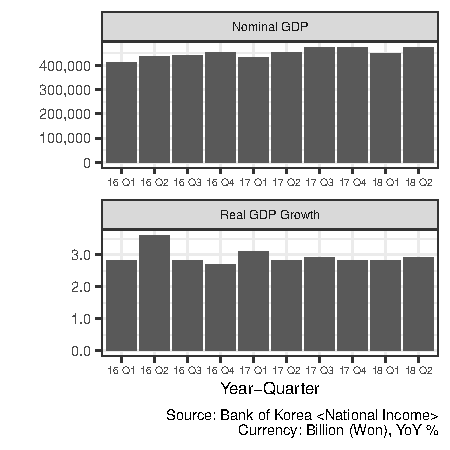
\includegraphics{manuscript_files/figure-latex/fig1-1} 

}

\caption{\label{fig1} Changes in Economic Size and Growh}\label{fig:fig1}
\end{figure}

Also, North Korea's provocation of South Korea is the kind of
conflictive event that can affect the attitudes of South Koreans toward
North Korea and unification; 2015 was a time of heightened military
tension in the inter-Korean relationship. On July 11, 2015, about 10
North Korean soldiers broke into the military demarcation line, and on
August 4, 2015, North Korea initiated a provocation that buried a mine
in the DMZ's western front. As a result, the South Korean government
warned North Korea and resumed the cross-border loudspeaker broadcasting
campaign it had waged against North Korea for the previous 11 years as a
punishment. In response, North Korea launched a shelling attack on
August 20 in Yeoncheon, Gyeonggi-do. To resolve the military conflict
triggered by North Korea's landmine provocations and artillery
bombardment, senior officials from both sides met August 22--25, and
drew up the ``August 25 Agreement'' to release the tensions between
South and North Korea. The August 25 agreement states that South Korea
would suspend loudspeaker broadcasting and cancel semi-exhibition
status. The agreement also requires North Korea to be cooperative about
family reunions and to encourage exchanges and collaboration at the
civilian level.

Since 2016, North Korea's military provocation has shown a sharp
increase. In particular, along with conventional military provocations,
North Korea conducted military provocations, such as the experiment of
strategic weapons; the fourth nuclear test; a missile launch experiment
at Gwangmyeongseong Lake on February 7; a submarine-launched ballistic
missile (SLBM) test launch on April 24 from the Sinpo-class submarine,
at least five Hwaseong 10 (Musdan) medium-range ballistic missile
launches; a test launch of the North Star ballistic missile (SLBM) from
a new submarine on August 24; and a nuclear test on September 9.

In 2017, North Korea continued the military provocation with a political
slogan that promises the construction of great power. South Korea then
announced a pledge to appease North Korea in the process of holding a
presidential election on May 9, but North Korea neglected it. Jong-Un
Kim's regime continued to provoke military tensions in South Korea, as
well as in the United States and Japan. In 2018, starting from the
Pyeongchang Winter Olympics, the atmosphere of reconciliation between
the two Koreas was created, and there was no North Korean missile
launch. Thus, North Korea expanded its military provocations from 2015
to 2017, and by 2018 it showed signs of easing the tensions. In other
words, the people of South Korea were exposed to the threat of North
Korea's provocation until April 27, 2018, when the Panmunjom Declaration
was announced. In sum, Figure \ref{fig1} and North Korea's military
provocation log show that it is difficult to observe the kind of
macroscopic changes that can cause rapid changes in the attitudes toward
North Korea and the unification of South Koreans, before and after the
Panmunjom Declaration.

\begin{figure}[htbp]

{\centering 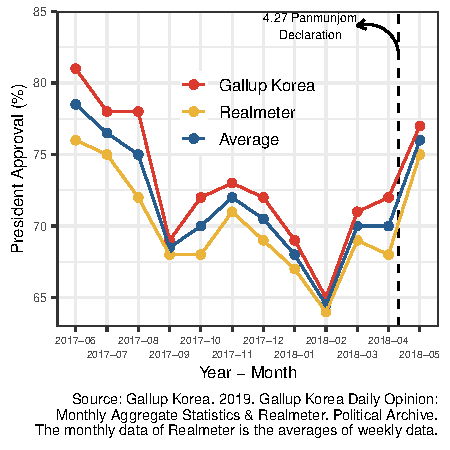
\includegraphics{manuscript_files/figure-latex/fig2-1} 

}

\caption{\label{fig2} Approval of President Jae-In Moon (June 2017-June 2018}\label{fig:fig2}
\end{figure}

On the contrary, Figure \ref{fig2} implies that the Panmunjom
Declaration may have a critical influence on the South Koreans. It shows
the monthly approval ratings of the presidential administration
conducted by Gallup Korea and Realmeter. According to Figure \ref{fig2},
President Jae-In Moon's approval rates continued to decline, beginning
in June 2016, and began sharply rebounding in February 2018. In February
2018, President Jae-In Moon and Yeo-Jung Kim, the vice director of the
Central Committee of the Workers' Party of North Korea, had a meeting.
Yeo-Jung Kim delivered a letter from Jong-Un Kim, chairman of the State
Council, and verbally asked President Jae-In Moon to visit Pyongyang.
This shows that the Panmunjom Declaration can be an influential event on
the attitudes toward North Korea and unification compared to other
events. Therefore, we will take a look at the discriminatory results
from previous studies that appeared through public surveys after the
Panmunjom Declaration in the context of the impact of political events.

\hypertarget{data}{%
\subsubsection{Data}\label{data}}

The data used in this paper is the Korean Broadcasting System (KBS)
National Unification Consciousness Survey of 2018 conducted by KBS
(hereafter, KBS survey). KBS surveyed for five days from August 3 to
August 7, 2018. It weighted population proportions by gender, age, and
region based on the registered population in July 2018. It is made up of
1,000 samples, valid for men and women over the age of 19 who live in
cities and provinces. The KBS survey contains questions on the attitude
toward North Korea in terms of leadership and general perception and
attitudes toward unification after the Panmunjom Declaration. Also, it
shows the least time difference from the Panmunjom Declaration.
Therefore, among the available survey data, it is the most suitable for
use in the empirical analysis for this study.

It should be noted that this is not panel data that surveys the same
respondents at different times. It is difficult to find significant
events that could affect the attitude toward North Korea and unification
at that time except for the Panmunjom Declaration. However, it does not
mean that we can interpret that the change after the Panmunjom
Declaration is due to the effect of the political event. It is necessary
to consider that there are no available panel surveys to analyze the
Panmunjom Declaration before-and-after. Hence, the KBS survey can be
helpful for an empirical analysis of the individual level of attitudes
toward North Korea and unification after the event, although the data
have several limitations. If we are not overconfident of the results of
the analysis, we can expect to find significant implications that will
help us understand the changing attitudes of South Koreans toward North
Korea and unification after the Panmunjom Declaration.

\hypertarget{dependent-variables}{%
\paragraph{Dependent Variables}\label{dependent-variables}}

\hypertarget{attitudes-toward-north-korea-leadership-and-general-state}{%
\paragraph{Attitudes toward North Korea: Leadership, and General
State}\label{attitudes-toward-north-korea-leadership-and-general-state}}

The dependent variables of interest are the attitudes toward North
Korea, and unification. We use two questions to classify the attitude
toward North Korea---North Korean leadership, or North Korea in general.
We expect attitudes toward North Korea to be differentiated into North
Korean leadership and North Korea as a general state. First, we look at
the question about North Korean leadership: ``What do you think of
Jong-Un Kim's North Korean regime and its ruling leadership group?'' The
responses on North Korean leadership were given on a five-points scale,
with 1 meaning ``very dissatisfied'' to 5, meaning ``very satisfied.''
Also, we asked the question, ``What do you think about North Korea?'' to
measure general attitudes toward North Korea. The responses are also
measured on a five-point scale from 1, ``I think North Korea is a
hostile entity,'' to 5, ``I think South Korea should support North
Korea.''

\begin{figure}[ht]

{\centering 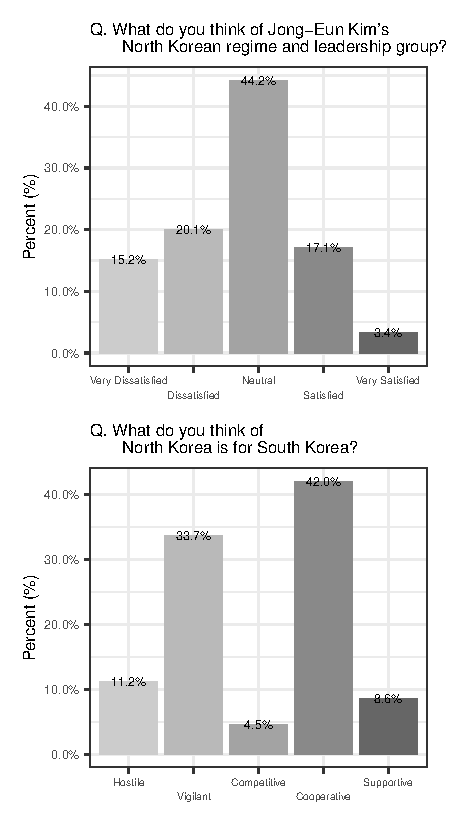
\includegraphics{manuscript_files/figure-latex/fig3-1} 

}

\caption{\label{fig3} The Distribution of Attitudes toward North Korea: Leadership, and General State}\label{fig:fig3}
\end{figure}

When we looked at the distribution of attitudes toward North Korea after
the Panmunjom Declaration, we can see that there is a difference between
the attitudes toward North Korean leadership and North Korea in general.
First, the responses on the North Korean leadership were mostly reserved
(``Neutral,'' 44.2\%). Otherwise, respondents showed a feeling of
antipathy (35.2\%) rather than favorability (20.5\%). Similarly,
respondents to the question of North Korea in general show that they
rarely think of North Korea as a competitor (4.5\%). It reflects the
perceptions of the political, economic, and social gaps between the two
Koreas that South Koreans have experienced for 70 years, which means
that North Korea is no longer competing against South Korea at the
system level. The most frequent response is to recognize North Korea as
a ``cooperative'' entity (42\%), followed by a view of being a
``vigilant'' entity (33.7\%). It confirms that after the Panmunjom
Declaration, respondents are still dissatisfied with the North Korean
leadership. At the same time, however, respondents perceive North Korea
as an inevitable entity with which to interact to solve the inter-Korean
relationship and other problems concerning the Korean peninsula.

\hypertarget{attitudes-toward-unification}{%
\paragraph{Attitudes toward
Unification}\label{attitudes-toward-unification}}

\begin{figure}[htbp]

{\centering 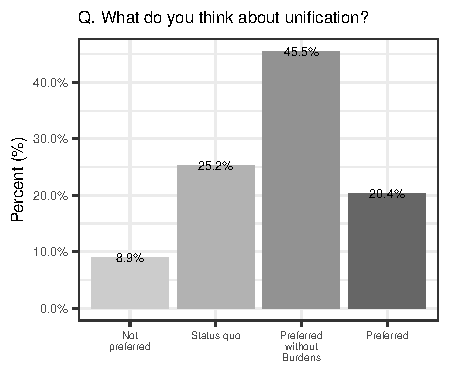
\includegraphics{manuscript_files/figure-latex/fig4-1} 

}

\caption{\label{fig4} The Distribution of Attitudes toward Unification}\label{fig:fig4}
\end{figure}

Figure \ref{fig4} shows the distribution of respondents about the
attitudes toward unification. We asked, ``What do you think about
unification?'' Responses were measured on a four-point scale. The most
frequent response is the opinion that respondents prefer unification if
it creates no burdens (45.5\%). Only 8.9\% of respondents say that they
do not prefer unification. A quarter of the respondents answer that they
prefer the status quo (25.2\%), and only 20.4\% say they prefer
unification unconditionally.

On the one hand, Figure \ref{fig4} implies that it is necessary to
examine in detail the burden of unification, a condition that
significantly affects attitudes toward unification. Figure \ref{fig5}
shows opinions about the burden of unification with the question, ``What
do you think is most worrying about the unification process?'' The
results indicate that the potential cost of unification are many
people's biggest concern.

\begin{figure}[htbp]

{\centering 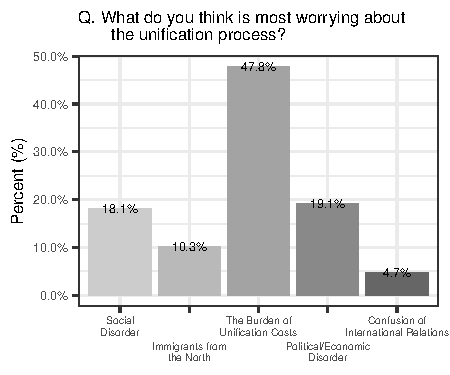
\includegraphics{manuscript_files/figure-latex/fig5-1} 

}

\caption{\label{fig5} Most Worrying about the Unification Process}\label{fig:fig5}
\end{figure}

Figure \ref{fig6} shows the distribution of respondents who answered
that the cost of unification is their biggest concern, and how much of
their annual income might be paid in taxes to cover the cost. About 28\%
of those who said that unification costs are the most significant
concern would refuse to personally subsidize unification costs
(28.24\%). Figure 6 also reveals that although respondents recognize
that the most crucial factor in unification is the cost, they are less
likely to pay for the costs by themselves. It can be said to show a
change in the perception of pragmatic rationality of unification
mentioned by previous studies \citep{ChoHan2014}.

\begin{figure}[htbp]

{\centering 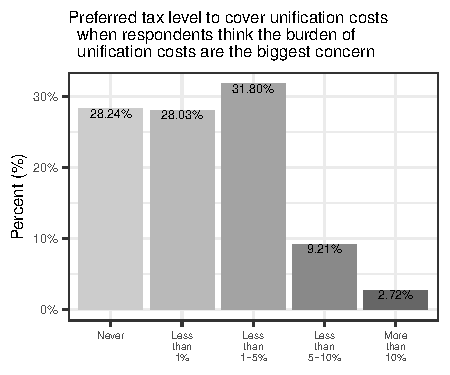
\includegraphics{manuscript_files/figure-latex/fig6-1} 

}

\caption{\label{fig6} Preferred Tax Level for Unification Costs Whose Biggest Concern is Unification Burden}\label{fig:fig6}
\end{figure}

\hypertarget{explanatory-variables}{%
\paragraph{Explanatory Variables}\label{explanatory-variables}}

One of the main explanatory variables in this study is generational. We
investigate how the generations are associated with the attitudes toward
North Korea and unification after the Panmunjom Declaration. Generations
are categorical variables measured in 10-year units based on age. The
younger generations, in their 20s and 30s, are those who experienced
several provocations of North Korea and the failure of appeasement
policies. It means that the Panmunjom Declaration may not be an event
critical enough to change their political attitude fundamentally.
Instead, the younger generation can accept the Panmunjom Declaration as
part of the repetitive North Korean warfare tactics.

Thus, we expect that the younger generations would persist in
conservative views on North Korea regardless of its leadership and
general perception. However, the older generations, in their 40s and
50s, who experienced the period of successful appeasement policies,
would expect that the Panmunjom Declaration will bring peace again.
Lastly, the oldest generation surveyed, those in their 60s and over, is
expected to show a negative attitude toward the leadership, but not as a
general perception. Since the oldest generation are those who
experienced the Korean War or its immediate aftermath, for them, North
Korea is both an enemy of the Korean War and, at the same time, belongs
to the same Korean nationality. Therefore, unlike the previous studies,
we expect a nonlinear relationship between different generations and
attitudes toward North Korean leadership. Conversely, the relationship
between generations and attitudes toward North Korea in general would
not be distinctive across the generations since South Koreans have
learned through a series of events that the people who are ruled in
North Korea do not influence the inter-Korean relationship. The
reference category among the generations are those in their 20s, who are
expected, in this survey, to show conservative or negative attitudes
toward North Korea even after the Panmunjom Declaration.

The other explanatory variable of interest is the prospect of
unification. This variable consists of responses to the question, ``When
do you think unification will happen?'' The longer the period of
unification, the more negative the prospect. It is because we can view
the negative responses for the expected unification period as a kind of
``time of hesitation'' that expects a transitional period, such as the
preparation period for unification, considering the burdens, costs, and
social problems that will arise from unification. Moreover, responses
that the time when unification is possible is ``near'' or ``impossible
for the long term'' means that the motivation and expectations for
unification are low \citep[82]{Jeong2013}.

Finally, we control for other variables that can potentially affect the
attitudes toward North Korea and unification. The variables include the
regions where respondents live, gender, education level, income level,
evaluations of North Korea policies under the Jae-In Moon
administration, all drawn from the KBS survey data. Conventional wisdom
asserts that regionalism has driven the outcomes of elections in the
post-democratization period in Korea \citep{Kim2008}. We have observed a
regional divide in which the electorate of the Youngnam and the Honam
regions were opposed. Even the Youngnam region is divided into two
parts: northern Youngnam, with the city of Daegu, and southern Youngnam,
with the cities of Pusan and Ulsan \citep{Kang2000, Kim2010, Yoon2012}.

Evaluations toward North Korea's policies under the Jae-In Moon
administration is a proxy variable of political ideology or party
identification, considered in previous studies. Political ideology
mostly measures the spectrum of liberal or conservative, and party
identification measures a respondent's attachment to a particular party
as a primary political variable. The political ideology or party
identification in current studies is used to explore the determinants of
attitudes toward North Korea and unification. However, the KBS survey
data used in this study do not include questions that directly measure
the political ideology or party identification of respondents. We expect
that the evaluations will show the ideological tendency because voters
in South Korea have shown significant differences in policy issues in
terms of North Korea support and the ROK-US alliance
\citep{Parketal2012}. Socio-demographic variables, such as gender,
education level, and income level, are also included.

\begin{figure}[htbp]

{\centering 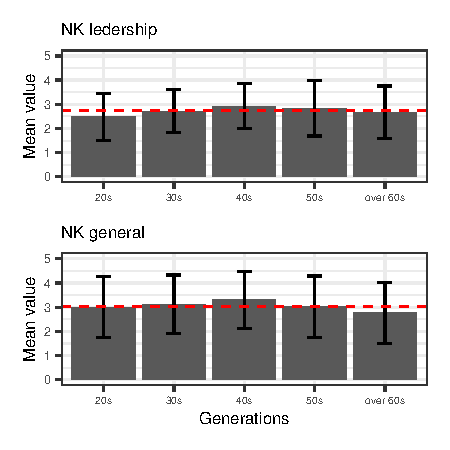
\includegraphics{manuscript_files/figure-latex/fig7-1} 

}

\caption{\label{fig7} Bivariate Relationship between Attitudes toward North Korea and Different Generations}\label{fig:fig7}
\end{figure}

\hypertarget{empirical-findings}{%
\subsection{Empirical Findings}\label{empirical-findings}}

\hypertarget{bivariate-analyses}{%
\subsubsection{Bivariate Analyses}\label{bivariate-analyses}}

Figure \ref{fig7} and Figure \ref{fig8} show preliminary bivariate
analyses. Figure \ref{fig7} is a bar plot where the x-axis represents
discrete generations, while the y-axis represents the mean value of the
attitudes toward North Korea. The red dashed line is the mean value of
the attitudes toward North Korean leadership and North Korea in general.
On average, Figure \ref{fig7} implies that respondents are more likely
to show a negative attitude toward North Korean leadership than North
Korea in general. In terms of the attitude toward North Korean
leadership, the youngest generation, in their 20s, show the lowest mean
value, which means that South Koreans in their 20s are more likely to
consider North Korean leadership negatively. Otherwise, people in their
40s have the highest mean value, which indicates that people in their
50s are more likely to feel familiar with North Korean leadership than
other generations. Figure 8 is about the attitude toward North Korea in
general. As expected, the generation of people 60 and over are more
likely to answer that they consider North Korea to be a hostile and
vigilant counterpart. Other generations show a positive attitude toward
North Korea in general compared to people 60 and over. In particular,
people in their 40s have the most positive attitude toward North Korea
in general across the generation groups. Thus, in terms of the
perceptions about leadership and North Korea in general, people in their
40s are the most generous group.

\begin{figure}[ht]

{\centering 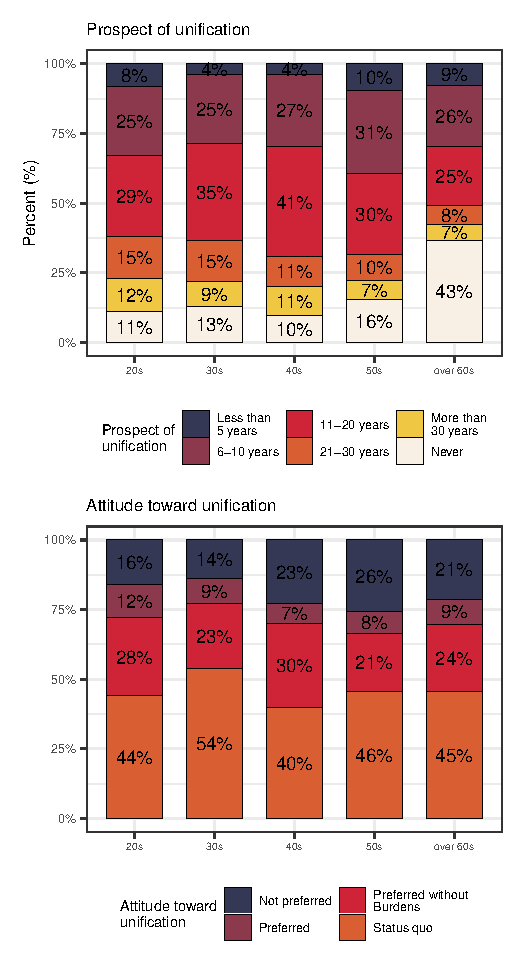
\includegraphics{manuscript_files/figure-latex/fig8-1} 

}

\caption{\label{fig8} Bivariate Relationship between Prospect of Attitudes toward Unification and Different Generations}\label{fig:fig8}
\end{figure}

Figure \ref{fig8} is a stacked bar plot that displays the bivariate
relationship of the variables regarding unification and generations. In
the left panel of Figure 8, the x-axis represents generations, while the
y-axis indicates the percentages of the answers of the prospect for
unification across generations. KBS survey data measures the prospect of
unification as a six-point scale. We can expect that the shorter the
prospect is, the more positive prospect it is for unification.

\begin{table}[H] \centering 
  \caption{Ordered Logistic Regressions: Attitudes toward North Korea after the Panmunjom Declaration} 
  \label{tab1} 
\begin{tabular}{@{\extracolsep{5pt}}lcc} 
\\[-1.8ex]\hline 
\hline \\[-1.8ex] 
 & \multicolumn{2}{c}{Attitudes toward North Korea} \\ 
\cline{2-3} 
 & Leadership & General \\ 
\hline \\[-1.8ex] 
 Generation: 30s & 0.313 & $-$0.041 \\ 
  & (0.203) & (0.206) \\ 
  & & \\ 
 Generation: 40s & 0.521$^{**}$ & 0.133 \\ 
  & (0.201) & (0.203) \\ 
  & & \\ 
 Generation: 50s & 0.574$^{**}$ & $-$0.110 \\ 
  & (0.208) & (0.206) \\ 
  & & \\ 
 Generation: 60+ & 0.403 & $-$0.182 \\ 
  & (0.209) & (0.209) \\ 
  & & \\ 
 Evaluation of the Govt.'s NK policy & 1.427$^{***}$ & 1.219$^{***}$ \\ 
  & (0.085) & (0.082) \\ 
  & & \\ 
 Region: Honam & $-$0.196 & 0.073 \\ 
  & (0.206) & (0.201) \\ 
  & & \\ 
 Region: PK & $-$0.049 & 0.095 \\ 
  & (0.167) & (0.172) \\ 
  & & \\ 
 Region: TK & $-$0.086 & $-$0.285 \\ 
  & (0.204) & (0.204) \\ 
  & & \\ 
 Socio-demografic: Gender & 0.595$^{***}$ & 0.386$^{**}$ \\ 
  & (0.122) & (0.121) \\ 
  & & \\ 
 Socio-demografic: Education & $-$0.266$^{*}$ & 0.032 \\ 
  & (0.122) & (0.123) \\ 
  & & \\ 
 Socio-demografic: Income & 0.174$^{**}$ & 0.170$^{**}$ \\ 
  & (0.054) & (0.055) \\ 
  & & \\ 
cut1 & 2.594 & 1.911 \\ 
 & (0.451) & (0.444) \\ 
cut2 & 4.071 & 4.319 \\ 
 & (0.462) & (0.464) \\ 
cut3 & 6.557 & 4.558 \\ 
 & (0.489) & (0.467 \\ 
cut4 & 8.785 & 7.307 \\ 
 & (0.524) & (0.497 \\ 
Log-likelihood ratio & 386.212 & 311.067 \\ 
Observations & 996 & 996 \\ 
\hline \\[-1.8ex] 
\textit{Note:}  & \multicolumn{2}{r}{$^{*}$p$<$0.05; $^{**}$p$<$0.01; $^{***}$p$<$0.001} \\ 
 & \multicolumn{2}{r}{Standard errors in parentheses.} \\ 
 & \multicolumn{2}{r}{PK/TK are abbreviations of the regions:} \\ 
 & \multicolumn{2}{r}{PK: Pusan/Ulsan/Kyeongnam} \\ 
 & \multicolumn{2}{r}{TK:Taegu/Kyeongbuk} \\ 
\end{tabular} 
\end{table}

The results show that the over-60s group is more likely to have a
skeptical prospect of unification. About 43\% of the respondents in the
over-60s group answer that unification will never come. People in their
50s (41\%) and 40s (31\%) are the generations that think unification
could happen in less than ten years. The right panel shows the
relationship between attitudes toward unification and generations. From
the right panel, we can see that ``prefer unification unconditionally''
had the fewest responses among the choices across all generations. It
backs up the argument of \citet{ChoHan2014} or \citet{Choi2016} that the
attitudes toward unification in South Korea have changed significantly
over time since the division in 1945.

The dependent variables are the attitudes toward North Korea and
unification, measured on a major five-point scale. Also, the variables
have a discrete, not continuous, ranking. Therefore, we use ordered
logistic regression to estimate the relationship between dependent
variables and explanatory variables. The results of ordered logistic
regression are natural logarithms of the odds ratio that show the
probability of selecting each category of the dependent variable.
Although coefficients of ordered logistic regression are in linear
forms, it implies the nonlinear relationship between explanatory
variables and the dependent variable. Hence, it is difficult to derive a
direct implication through the coefficients. In this study, we show the
effects of the explanatory variables on the dependent variable as
marginal effects.

\hypertarget{attitudes-toward-north-korea-after-the-panmunjom-declaration}{%
\subsubsection{Attitudes toward North Korea after the Panmunjom
Declaration}\label{attitudes-toward-north-korea-after-the-panmunjom-declaration}}

Table \ref{tab1} is the result of examining the determinants of North
Korea's perception through ordered logistic regression analysis for
respondents after the Panmunjom Declaration. In Model 1, respondents of
all generations except those in their 30s were more likely to show more
positive attitudes toward North Korean leadership compared to those in
their 20s when we hold other explanatory variables constant. In other
words, we can understand that the 20s and 30s are more likely to show
negative attitudes and antipathy toward the North Korean leadership than
other generations. Model 2 analyzes the determinants of North Korea in
general. We cannot find any significant differences among generations
compared to those in their 60s and older in terms of attitudes toward
North Korea in general in Model 2. According to Figure 7, the bivariate
analysis tells South Koreans in their 20s, 30s, and 50s do not show
distinctive features. The 40s have a higher value than the average,
which implies that people in their 40s are more likely to answer the
question positively. People in their 60s have a lower value than
average, which means that they are more likely to be negative toward
North Korea in general. Although we changed the reference category from
people in their 20s to those over 60, we cannot find statistically
significant differences across the generations in terms of the attitudes
toward North Korea in general.

\begin{figure}[ht]

{\centering 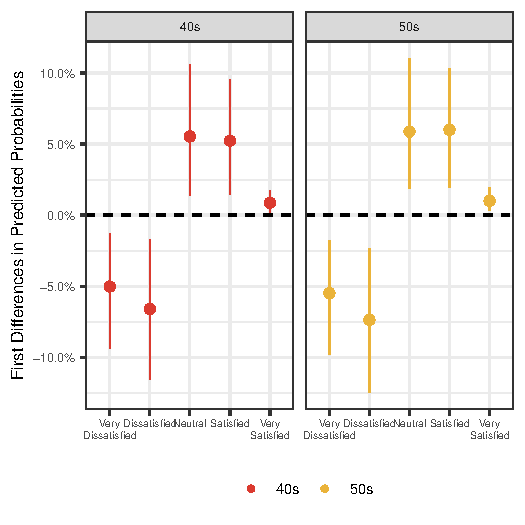
\includegraphics{manuscript_files/figure-latex/fig9-1} 

}

\caption{\label{fig9} First Differences in Predicted Probabilities}\label{fig:fig9}
\end{figure}

Figure \ref{fig9} reports changes in the predicted probability of the
dependent variable when a statistically significant independent variable
increases by changes from 0 to 1, holding all other variables constant.
The study's results support the hypothesis that younger generations (in
their 20s and 30s) show a more conservative attitude toward North Korea
and unification than other generations even after the Panmunjom
Declaration. Those who belong to the older generations (in their 40s)
are significantly more likely to be satisfied with the North Korean
leadership. Explicitly, compared to those in their 20s, the probability
of people in their 40s saying they are very dissatisfied with the North
Korean leadership decreased 5.4\%, holding other variables constant at
their means. Also, the probability of people in their 40s saying they
are very satisfied increased by 1.5\% compared to people in their 20s.
From the 40s to the \(\geq\text{60s}\), they show a similar tendency for
attitudes toward North Korean leadership compared to people in their
20s.

\hypertarget{attitudes-toward-unification-after-the-panmunjom-declaration}{%
\subsubsection{Attitudes toward Unification after the Panmunjom
Declaration}\label{attitudes-toward-unification-after-the-panmunjom-declaration}}

Table \ref{tab2} examines the competing hypotheses about attitudes
toward unification from previous studies, and the second hypothesis,
that the prospects of unification affect the attitudes toward
unification differently across generations. In particular, we break down
the second hypothesis into two statements. First, the more positive the
prospects for unification, the more likely it is that older generations
will prefer unification. Secondly, the younger generations will not
change their attitudes toward unification even they have a positive
outlook on unification, since they have experienced the failure of
appeasement policies and repeated North Korean provocation.

Model 3 is a basic model composed of variables that can influence
attitudes toward unification derived from previous studies. Model 3
includes demographic variables, as well as variables that indicate the
degree of interest in unification, and evaluation of the current
government's policy toward North Korea policy. Respondents showed that
the higher the interest in unification, the more they prefer
unification. Likewise, the more supportive the current government's
policy is toward North Korea, the more likely people will respond that
they prefer unification. Model 4 shows the influence of generations on
attitudes toward unification. Since the reference group is people in
their 20s, we can interpret the results as effects of generations in
comparison with those in their 20s on attitudes toward unification after
the Panmunjom Declaration. Unlike previous studies, all generations did
not show statistically significant differences from people in their 20s.
Previous studies point out that the younger generations, such as those
in their 20s and 30s, tend to prefer unification less, since the
generations are more likely to approach unification issues with a view
to utility maximization rather than historical nationalism, and will
feel that unification is not practical \citep{ChoHan2014}. However,
after the Panmunjom Declaration, the generations do not show statistical
differences between each other, which are contrary to previous studies.

\begin{table}[!htbp] \centering 
  \caption{Ordered Logistic Regressions: Attitudes toward North Korea after the Panmunjom Declaration} 
  \label{tab2} 
\begin{tabular}{@{\extracolsep{5pt}}lcccc} 
\\[-1.8ex]\hline 
\hline \\[-1.8ex] 
 & \multicolumn{4}{c}{Attitudes toward Unification} \\ 
\cline{2-5} 
 & Base & Generation & Prospects & Full \\ 
\hline \\[-1.8ex] 
 30s &  & 0.137 &  & 1.239$^{*}$ \\ 
  &  & (0.209) &  & (0.619) \\ 
  & & & & \\ 
 40s &  & 0.057 &  & $-$0.118 \\ 
  &  & (0.206) &  & (0.633) \\ 
  & & & & \\ 
 50s &  & 0.304 &  & 1.971$^{**}$ \\ 
  &  & (0.211) &  & (0.604) \\ 
  & & & & \\ 
 60+ &  & 0.307 &  & 1.787$^{***}$ \\ 
  &  & (0.217) &  & (0.535) \\ 
  & & & & \\ 
 Prospects &  &  & 0.421$^{***}$ & 0.693$^{***}$ \\ 
  &  &  & (0.049) & (0.117) \\ 
  & & & & \\ 
 Interests & 1.247$^{***}$ & 1.230$^{***}$ & 1.085$^{***}$ & 1.090$^{***}$ \\ 
  & (0.092) & (0.093) & (0.094) & (0.095) \\ 
  & & & & \\ 
 NK policy Eval. & 0.657$^{***}$ & 0.672$^{***}$ & 0.498$^{***}$ & 0.515$^{***}$ \\ 
  & (0.081) & (0.083) & (0.084) & (0.086) \\ 
  & & & & \\ 
 Honam & $-$0.220 & $-$0.232 & $-$0.156 & $-$0.188 \\ 
  & (0.212) & (0.211) & (0.215) & (0.215) \\ 
  & & & & \\ 
 PK & $-$0.044 & $-$0.046 & $-$0.017 & $-$0.023 \\ 
  & (0.172) & (0.172) & (0.173) & (0.175) \\ 
  & & & & \\ 
 TK & 0.049 & 0.039 & 0.140 & 0.103 \\ 
  & (0.205) & (0.205) & (0.207) & (0.209) \\ 
  & & & & \\ 
 Gender & $-$0.144 & $-$0.151 & $-$0.252$^{*}$ & $-$0.291$^{*}$ \\ 
  & (0.123) & (0.123) & (0.125) & (0.126) \\ 
  & & & & \\ 
 Education & $-$0.013 & 0.064 & $-$0.028 & 0.065 \\ 
  & (0.111) & (0.123) & (0.113) & (0.125) \\ 
  & & & & \\ 
 Income & $-$0.044 & $-$0.041 & $-$0.080 & $-$0.071 \\ 
  & (0.054) & (0.055) & (0.055) & (0.056) \\ 
  & & & & \\ 
 30s$\times$Prospects &  &  &  & $-$0.284 \\ 
  &  &  &  & (0.158) \\ 
  & & & & \\ 
 40s$\times$Prospects &  &  &  & 0.033 \\ 
  &  &  &  & (0.158) \\ 
  & & & & \\ 
 50s$\times$Prospects &  &  &  & $-$0.443$^{**}$ \\ 
  &  &  &  & (0.149) \\ 
  & & & & \\ 
 60s$\times$Prospects &  &  &  & $-$0.375$^{**}$ \\ 
  &  &  &  & (0.134) \\ 
  & & & & \\ 
cut1 & 2.404 & 2.777 & 2.636 & 4.109 \\ 
 & (0.405) & (0.474) & (0.412) & (0.617) \\ 
cut2 & 4.543 & 4.914 & 4.916 & 6.435 \\ 
 & (0.422) & (0.488) & (0.433) & (0.638) \\ 
cut3 & 7.123 & 7.504 & 7.625 & 9.187 \\ 
 & (0.455) & (0.52) & (0.47) & (0.669) \\ 
Log-likelihood ratio & 377.507 & 380.96 & 455.642 & 479.648 \\ 
Observations & 996 & 996 & 996 & 996 \\ 
\hline \\[-1.8ex] 
\textit{Note:}  & \multicolumn{4}{r}{$^{*}$p$<$0.05; $^{**}$p$<$0.01; $^{***}$p$<$0.001} \\ 
 & \multicolumn{4}{r}{Standard errors in parentheses.} \\ 
\end{tabular} 
\end{table}

Model 5 analyzes the relationship between the prospect for and the
attitudes toward the unification. The longer the expected period of
unification is, the more negative the prospect is, because we can
consider it a transitional period. In other words, the expected period
for unification is not only the preparation period for unification, but
also the time of hesitation when we take into account the burdens,
costs, and social issues that will arise from unification. Moreover, the
response that the time when unification is possible is near or
impossible for the long term means that motivation and expectations for
unification are low \citep[82]{Jeong2013}. In Model 5, respondents
display negative attitudes toward unification as they are more cynical
about the prospect for unification, which was statistically significant.

\begin{figure}[htbp]

{\centering 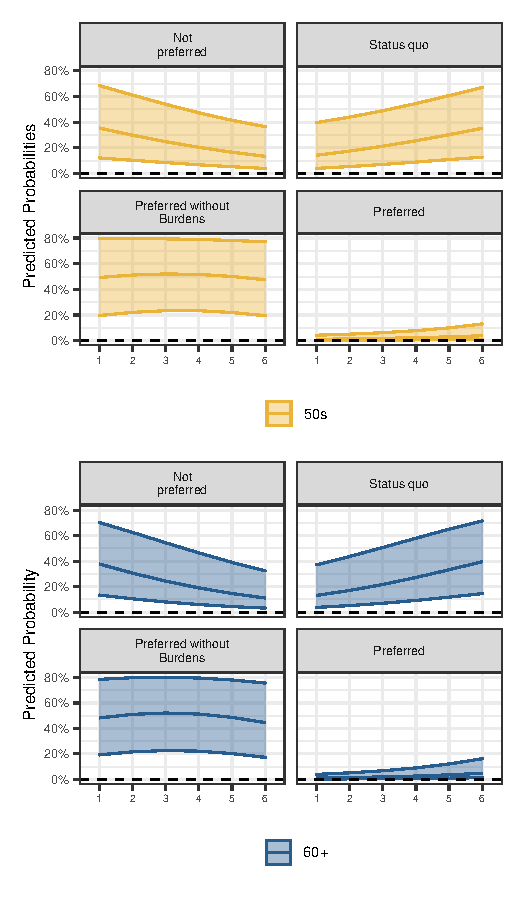
\includegraphics{manuscript_files/figure-latex/fig10-1} 

}

\caption{\label{fig10} Predicted Probabilities of the 40s and 50s}\label{fig:fig10}
\end{figure}

Lastly, we constructed Model 6 to test the second research hypothesis.
When the Panmunjom Declaration brings about fundamental changes in
recognition of unification by respondents, we expect that the more
positive the prospects for unification are, the more likely the
generations who have experienced past cooperative events will show
positive attitudes toward unification. Alternatively, respondents may
accept the Panmunjom Declaration as a part of North Korea's
stick-and-carrot strategy, not as a substantial change in the benefits
and costs of unification. We examine the interactions between the two
variables on the dependent variable by changing the prospects for
unification by the predicted probability in Figure \ref{fig10}.

Although Model 6 presents that the 50s and 60s are statistically
different from the 20s, Figure \ref{fig10} and Figure \ref{fig11} show
the details, which we need to think about their implications. When the
prospects become positive, all generations show similar patterns that
they are more likely to prefer unification, and less likely to oppose to
it. However, the 50s and 60s are different in terms of the answer of
``preferred without burdens.'' The 50s and 60s do not show much
variations by varying prospects of unification (Figure \ref{fig10}),
while the 20s, 30s and the 40s show greater variations as the prospects
become positive (Figure \ref{fig11}).

\begin{figure}[htbp]

{\centering 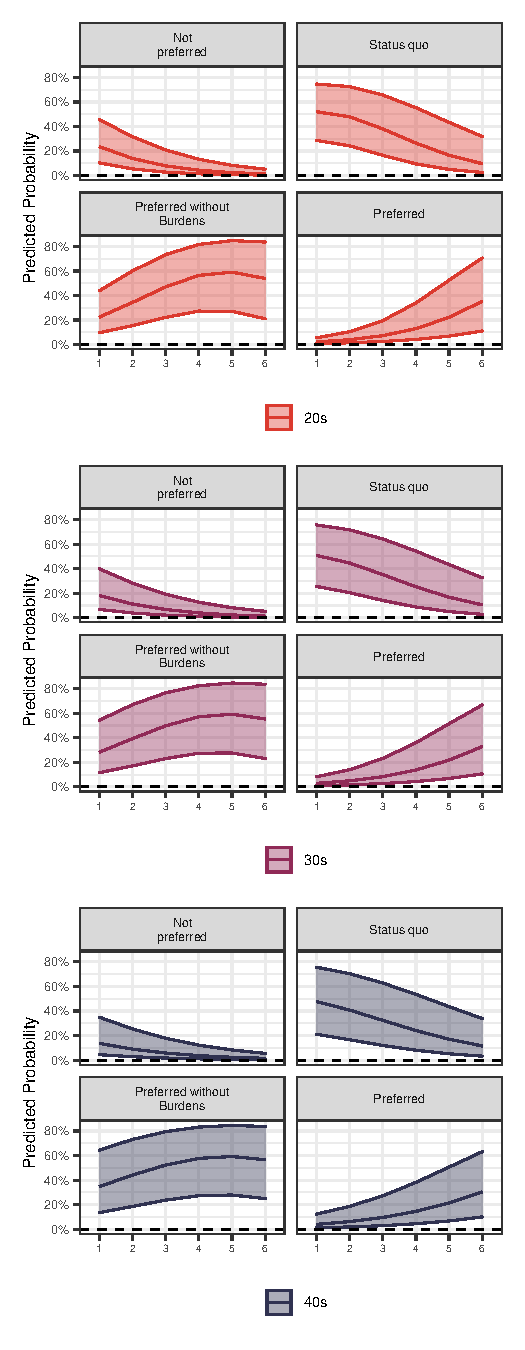
\includegraphics{manuscript_files/figure-latex/fig11-1} 

}

\caption{\label{fig11} Predicted Probabilities of the 20s, 30s, 60s}\label{fig:fig11}
\end{figure}

\hypertarget{conclusion-and-implications}{%
\subsection{Conclusion and
Implications}\label{conclusion-and-implications}}

This study investigates the attitudes toward North Korea and unification
based on data from the KBS National Unification Consciousness Survey of
2018. From the data, the generations who feel the most opposition to
North Korean leadership appear to be people in their 20s and 30s.
However, people in their 20s perceive North Korea in general to be
relatively moderate. It tells us that people in their 20s have the most
substantial attitudinal gap between the leadership and their perception
of North Korea in general.

The generational change also appears in the analysis of attitudes toward
unification after the Panmunjom Declaration. Variables such as the
degree of interest in unification, and the evaluation of current
governmental North Korea politics, are consistently related to the
attitude toward unification, but generational variables have different
impacts on unification preferences across the generations. For instance,
people in their 30s, 50s, and 60s and above are more likely to prefer
unification conditional on increasing positive prospects of unification
compared to people in their 20s. In other words, people in their 20s
became the generation that least prefers unification across the
generations. However, when we compared people in their 20s to people in
their 40s in Table 4, it shows that the tendency of both are similar in
changes of predicted probabilities. It implies that the 20s are the
generation that shows the most negative attitudes toward North Korea
leadership and unification; their attitudes are not static, but
conditional to the external environment, such as the change in
inter-Korean relationships.

We focus on the effect of the Panmunjom Declaration and attempt to
verify whether it had a positive effect on the prospects for future
unification like the previous inter-Korean cooperation cases. If
respondents from all generations improved in their attitude toward
unification as the unification prospects change after the Panmunjom
Declaration, we could expect that the declaration is the event that has
brought about a significant change in unification. However, it is
difficult to say that the event improves the prospects of unification
(Figure \ref{fig10} and Figure \ref{fig11}), and people in their 20s
show consistent negative attitudes toward North Korean leadership and
unification. In terms of unification, in particular, even when the
prospects of unification increase, people in their 20s are more likely
to have the most negative attitudes toward unification on average. In
particular, the younger generations and the 40s seem to estimate the
costs and benefits by the extent to the expected unification timing.

The changes, which are difficult to find in previous studies, clearly
show that the generation of our society is changing its attitude toward
North Korea and unification issues. Generational changes have been
observed as fragmentary events since 2017. For example, the strong
antipathy from people in their 20s and 30s over the 2018 Pyeongchang
Winter Olympics over the formation of the single inter-Korean women's
ice hockey team was challenging to find before that. Similarly, this
paper also consistently showed a negative attitude toward North Korea
and unification from the younger generation, which can be said to
capture the facets of generational changes in our society.

The results of this study show that the significant events driving
changes in inter-Korean relations can be made on the supply side, but we
should also pay attention to the changes that appear in the ordinary
people, who are the consumers, and other parties of the inter-Korean
relationship. The changes after the Panmunjom Declaration suggest that
the people who experience essential events in the inter-Korean
relationship form significantly different attitudes or prospects for
North Korea and unification. Thus, the government, as a supplier in the
unification and North Korea issues, not only provides one-sided policy
options but should also embrace the people's perceptions and attitudes,
which are sensitive to changes in the real world. At the same time, to
establish the justification logic of unification based on generational
changes, it is necessary to ensure long-term consistency in at least
unification and North Korea policy. Without policy consistency, citizens
cannot set the expected costs and benefits of unification to their
standards, which will make people anxious because of the uncertainty of
inter-Korean relations.

Lastly, we should note that the Panmunjom Declaration is a prominent
political event, but we do not need to overestimate it. The agreement
between the Panmunjom Declaration and the September 19 Pyongyang Joint
Declaration made significant progresses in many areas. However, the two
Koreas seem at a standstill, as the second North American summit in
Hanoi in February 2019 concluded without much success. Although South
Korea has long held political discussions related to North Korea and
unification since the division, we could not solve the fundamental
problem. Political leaders should consider public opinion to secure the
driving force for solving unification and North Korea problems. In
particular, in order to fundamentally change the perception toward North
Korea and unification, a domestic effort to supplement it is urgently
needed---not a one-off event.

%\showmatmethods


\bibliography{parkhur2020}
\bibliographystyle{jss}



\end{document}
